

The success of a mixed finite element formulation crucially depends on a proper choice of the local interpolations of the velocity and the pressure. 

%----------------------------------------------------------------------
\subsection{The compatibility condition (or LBB condition)}
\index{LBB} \index{optimal rate}

'LBB stable' elements assure the existence of a unique solution 
and assure convergence at the optimal rate. 

%----------------------------------------------------------------------
\subsection{Families}

\index{Taylor-Hood}

The family of Taylor-Hood finite element spaces on triangular/tetrahedral 
grids is given by $P_k \times P_{k-1}$ with $k\geq 2$, 
and on quadrilateral/hexahedral grids by $Q_k \times Q_{k-1}$ with $k\geq 2$.
This means that the pressure is then approximated by continuous functions. 

These finite elements are very popular, in particular the pairs for $k=2$, i.e.
$Q_2\times Q_1$ and $P_2\times P_1$.
The reason why $k\geq 2$ comes from the fact that the 
$Q_1 \times Q_0$ (i.e. $Q_1 \times P_0$) and $P_2\times P_1$
are not stable elements (they are not inf-sup stable). 

\begin{remark}
Note that a similar element to $Q_2 \times Q_1$ has been proposed
and used succesfully used \cite{taho73,hota74}: it is denoted by $Q_2^{(8)} \times Q_1$ 
since the center node ('$x^2y^2$') and its associated degrees of freedom have been removed. It 
has also been proved to be LBB stable. 
\end{remark}


\subsection{The bi/tri-linear velocity - constant pressure element ($Q_1\times P_0$)}

\includegraphics[width=3cm]{images/under_construction}

discussed in example 3.71 of \cite{john16}

However simple it may look, the \index{$Q_1 \times P_0$} element is 
one of the hardest elements to analyze and many questions are still open about its properties. 
The element does not satisfy the inf-sup condition \cite{hugh}p211. 
In \cite{grsa} it is qualified as follows: slightly unstable but highly usable. 

The $Q_1 \times P_0$ mixed approximation is the lowest order conforming approximation 
method defined on a rectangular grid. It also happens to be the most famous example 
of an unstable mixed approximation method.
\cite[p235]{elsw}.

This element is discussed in \cite{fort81}, \cite{fofo85} and in \cite{pisa85} 
in the context of multigrid use.

This element is plagued by so-called pressure checkerboard modes which
have been thoroughly analysed \cite{grsi94}, \cite{chpc95}, \cite{sagl81a,sagl81b}.
These can be filtered out \cite{chpc95}. Smoothing techniques are also discussed in \cite{legs79}.





%----------------------------------------------------------------------
\subsection{The bi/tri-quadratic velocity - discontinuous linear pressure element ($Q_2 \times P_{-1}$)}

\includegraphics[width=3cm]{images/under_construction}

This element is crowned "probably the most accurate 2D element" in \cite{grsa}.


%----------------------------------------------------------------------
\subsection{The bi/tri-quadratic velocity - bi/tri-linear pressure element ($Q_2 \times Q_1$)}

\includegraphics[width=3cm]{images/under_construction}

In \cite{grsa} Gresho \& Sani write that in their opinion $div(\vec v)=0$ is not strong enough.

This element, implemented in penalised form, is discussed in \cite{been79} and the follow-up paper \cite{been80}. CHECK

Biquadratic velocities, bilinear pressure. See Hood and Taylor. The element satisfies the inf-sup condition \cite{hugh}p215. 

\begin{center}
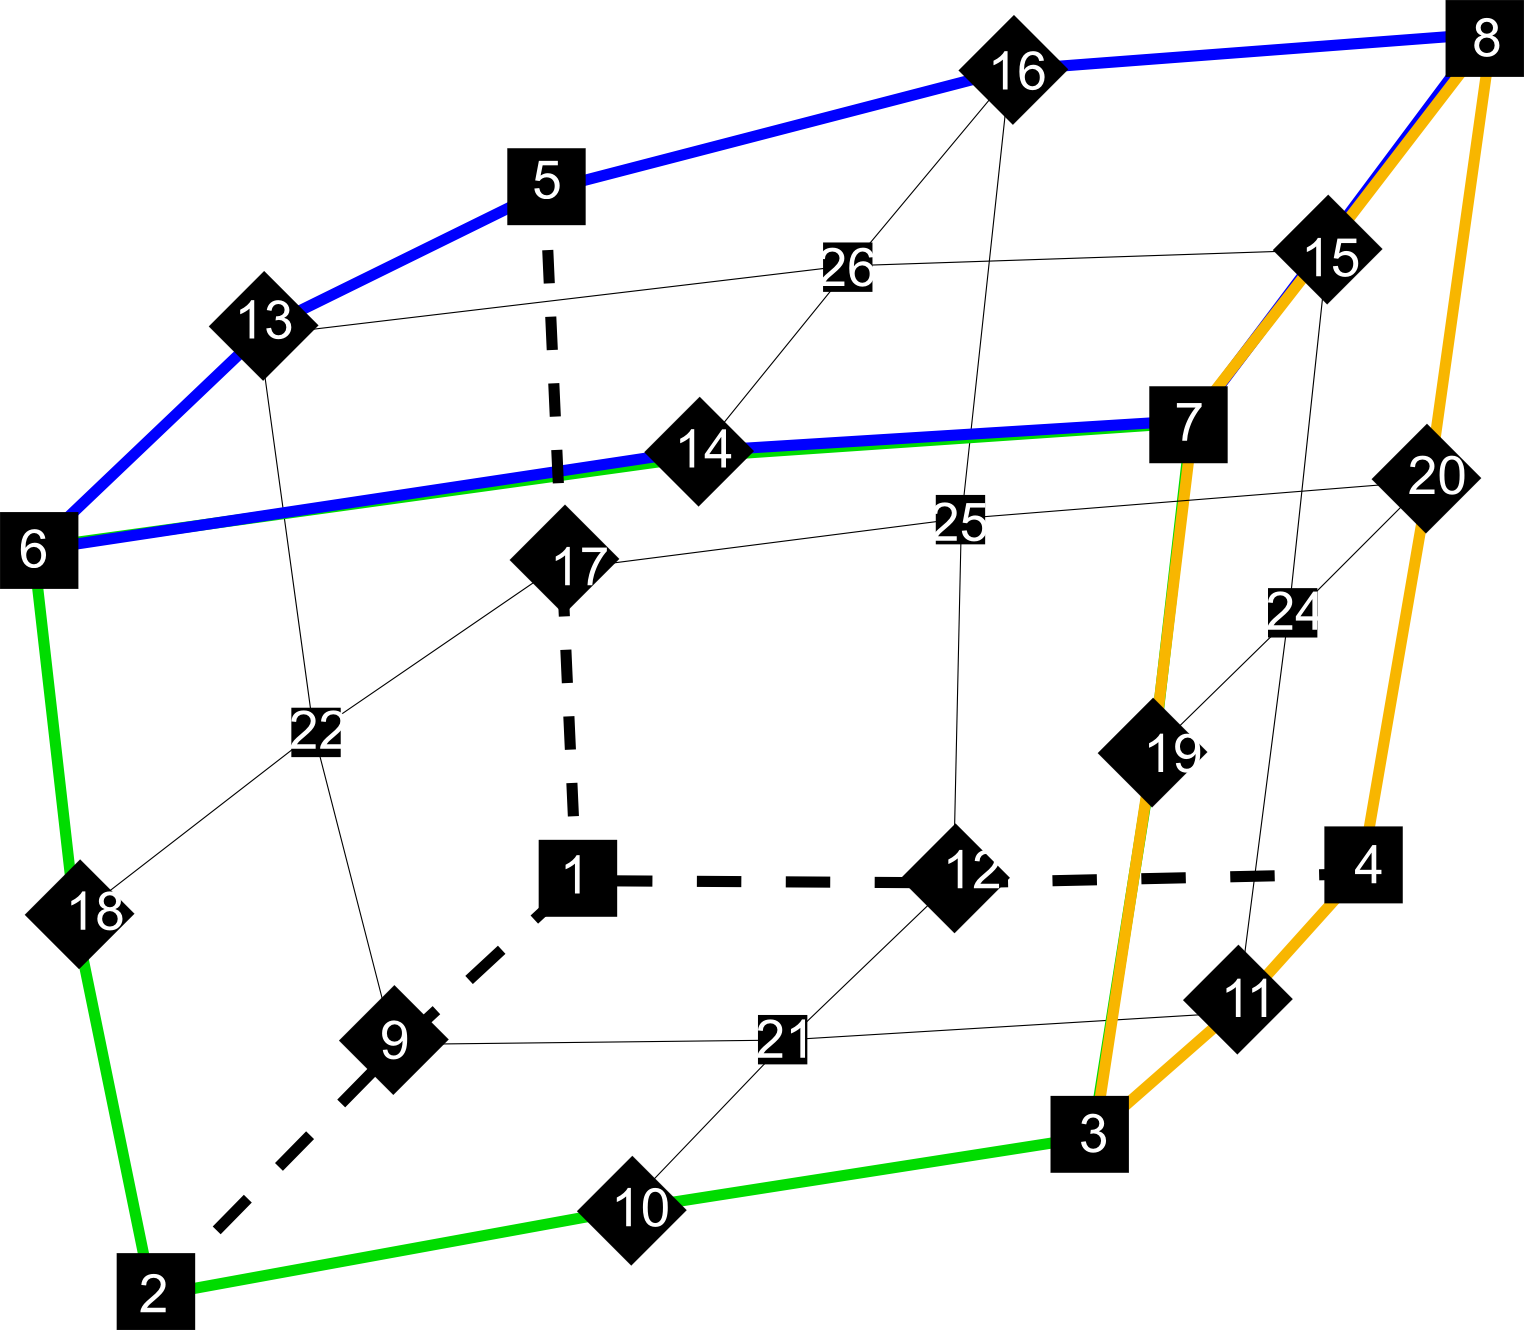
\includegraphics[width=6cm]{images/q2q1/q2numering}
\end{center}


%----------------------------------------------------------------------
\subsection{The stabilised bi/tri-linear velocity -  bi/tri-linear pressure element ($Q_1\times Q_1$-stab)}

\includegraphics[width=3cm]{images/under_construction}

%----------------------------------------------------------------------
\subsection{The MINI triangular element ($P_1^+\times P_1$)}

\includegraphics[width=3cm]{images/under_construction}

discussed in section 3.6.1 of \cite{john16}

%----------------------------------------------------------------------
\subsection{The quadratic velocity - linear pressure triangle ($P_2\times P_1$)}

\includegraphics[width=3cm]{images/under_construction}

From \cite{segal}.
Taylor-Hood elements (Taylor and Hood 1973) 
are characterized by the fact that the pressure is continuous in the region $\Omega$. 
A typical example is the quadratic triangle (P2P1 element).
In this element the velocity is approximated by a quadratic polynomial and the pressure by a
linear polynomial. One can easily verify that both approximations are continuous over 
the element boundaries. 
It can be shown, Segal (1979), that this element is admissible if at least 3 elements 
are used. The quadrilateral counterpart of this triangle is the $Q_2\times Q_1$ element.




%----------------------------------------------------------------------
\subsection{The Crouzeix-Raviart triangle ($P_2^+\times P_{-1}$)}

\includegraphics[width=3cm]{images/under_construction}

This element was first introduced in \cite{crra73}.

From \cite{daks08}: seven-node Crouzeix-Raviart triangle with quadratic velocity shape functions enhanced by a cubic bubble function and discontinuous linear interpolation for the pressure field [e.g., Cuvelier et al., 1986]. This element is stable and no additional stabilization techniques are required [Elman et al., 2005].

From \cite{segal}. These elements are characterized by a discontinuous pressure; 
discontinuous on element boundaries. 
For output purposes (printing, plotting etc.) these discontinuous pressures are averaged 
in vertices for all the adjoining elements.

The most simple Crouzeix-Raviart element is the non-conforming linear triangle 
with constant pressure ($P_1\times P_0$).

p248 of Elman book. satisfies LBB condition. 


This element is characterized by a discontinuous pressure; 
so that for output purposes (printing, plotting etc.) 
these discontinuous pressures are averaged in vertices for all the adjoining elements. 








%-----------------------------------------------------------------
\subsection{The Rannacher-Turek element - rotated $Q_1\times P_0$}

p. 722 of \cite{john16}

%----------------------------
\subsection{Other elements}

\begin{itemize}
\item P1P0 example 3.70 in \cite{john16}
\item P1P1
\item Q2P0: 
\index{$Q_2 \times P_0$} 
Quadratic velocities, constant pressure. The element satisfies the inf-sup condition, but the constant pressure assumption may require fine discretisation.

\item Q2Q2: This element is never used, probably because a) it is unstable, b) it is very costly. 
There is one reference to it in \cite{hufb86}.
\item P2P2
\item the MINI quadrilateral element $Q_1^+\times Q_1$. \index{$Q_1^+ \times Q_1$} 
\end{itemize}

